% adapted by WS from SSR's Word document and from the 5-part series at
% https://www.overleaf.com/learn/latex/How_to_Write_a_Thesis_in_LaTeX_(Part_1):_Basic_Structure
% reviewed by MAM

\documentclass[12pt,twosided]{report}

\usepackage[titletoc]{appendix} % for adding appendix to TOC
\usepackage[sorting=none]{biblatex}  % reference management
\usepackage{geometry}  % better margins and margin control
\usepackage{graphicx}  % to include figures
\usepackage{hyperref}  % internal and external links
\usepackage[utf8]{inputenc}  % support for non-ASCII characters
\usepackage{listings}  % typset code
\usepackage{outlines}  % easy nesting of lists
\usepackage{tabularx}  % more control over table column width
\usepackage{titlesec}  % customize chapter title 
\usepackage{upquote}  % prevent mishandling of single quotes in listings


% TODO: Customize the appearance of hyperref links using \hypersetup
% See https://en.wikibooks.org/wiki/LaTeX/Hyperlinks#Customization

% Custom format of chapter title.
\titleformat{\chapter}[hang]{\bf\huge}{\thechapter.}{2pc}{}

% Separate folder for images named 'images'.
\graphicspath{ {images/} }

% Separate file for references
\addbibresource{references.bib}

% Replace with your title
\title{Personalized Outfit Recommendation System}

% Allow recalling document title
% from https://tex.stackexchange.com/a/15806/44301
\makeatletter\let\Title\@title\makeatother  

\begin{document}

\begin{titlepage}
  
  \newgeometry{top=100pt,bottom=75pt}   
  \begin{center}
    \vfill
    \textbf{\Huge \Title}
    \bigskip

    {\large Kaavish Report\\
      presented to the academic faculty\\
      by\\\bigskip
      \begin{tabular}{ll}
        Muhammad Ali & ma02526\\
        Osama Yousuf & oy02945\\
        Syeda Areeba Kazmi & sk02901\\
        Tasneem Adnan & ta02903\\
      \end{tabular}
    }\\\vfill
    \includegraphics[width=.4\textwidth]{logo.pdf}\\
    {\large In partial fulfillment of the requirements for\\
      \textit{Bachelor of Science}\\
      Computer Science\\\medskip
      \textbf{Dhanani School of Science and Engineering}\\\medskip
      Habib University\\\smallskip
      Spring 2020
    }\\\vfill
    Copyright {\scriptsize \textcopyright} 2019 Habib University
  \end{center}
  \restoregeometry
\end{titlepage}

%%% Local Variables:
%%% mode: latex
%%% TeX-master: "report"
%%% End:
  % title page.
\thispagestyle{empty}
\centerline{\textbf{\LARGE \Title}}
\vfill

This Kaavish project was supervised by:\\\bigskip\\\bigskip\\\bigskip

% TODO: Use the appropriate table below depending on whether you have an external advisor. Comment out the unused table.

% If no external supervisor.
\hfill %
\begin{tabular}{l}
  \line(1,0){200}\\
  Dr. Shahid Hussain \\ 
  Faculty of Computer Science\\
  Habib University
\end{tabular}\\\bigskip\bigskip

% % If external supervisor.
% \begin{tabularx}{\linewidth}{lXl}
%   \line(1,0){175} & & \line(1,0){175}\\  % Signatures.
%   My External Supervisor & & My Internal Supervisor \\ % Names of your supervisors
%   Designation & & Faculty of Computer Science\\  % External supervisor's role/job tile at their company.
%   Awesome Ltd. & & Habib University  % External supervisor's company.
% \end{tabularx}\\\bigskip\bigskip

Approved by the Faculty of Computer Science on \hrulefill.

%%% Local Variables:
%%% mode: latex
%%% TeX-master: "report"
%%% End:
  % approval page.

\chapter*{Dedication}
For ammi, abbu, and pappu.

\chapter*{Acknowledgements}
We want to thank the CS faculty and ...

\chapter*{Abstract}
Abstract goes here

% The following are automatically populated by LaTeX \chapter, \section and related, \figure, and \table.
\tableofcontents
\listoffigures
\listoftables

% TODO: Put chapters in a separate folder named 'chapters'.

\chapter{Introduction}
\label{chap:intro}
\section{Problem Statement}

\textbf{\emph{Domain:}} Fashion e-commerce. \\\\
\textbf{\emph{Facts and Figures:}} 
\begin{enumerate}
	\item Personalized shopping is the future of commerce. It is reported that on average today, at least 27\% of retail site revenue in fashion, which totals to around \$870 million, comes from personalized recommendations systems. \cite{salesforce}
	\item In 2013, over 85\% of Amazon sales revenue came through personalized recommendations. \cite{mckinsey}
	\item Despite all its potential, the Pakistani fashion industry is lagging behind in keeping up with such advances in personalized recommendation systems. \cite{thenewspk}
\end{enumerate}
\textbf{\emph{Statement:}} One of the biggest problems in fashion retail is product curation. Retailers have to spend a large amount of time to come up with different combinations of their products that would as a whole, go well as an outfit, and even then, the options aren’t really personalized. A customer buys a new shirt, brings it home, and hangs it up, only to find that the shirt stays in their closet for weeks because they’re not sure what to pair it with. This also means a loss in conversion rates and potential revenue at the side of the retailer.

\section{Proposed Solution}

As already described, fashion retailers spend a lot of time manually curating their products, and according to a report published by emerj.com (database of reports on AI technology), at least 40\% of potential revenues are lost because of poor outfit recommendations. We see a business opportunity in this problem, and so the idea behind the project is to solve it by addressing the key issue, product curation, by providing expert recommendations across different clothing items to the end-consumer at the point of sale or as a standalone service.


Our solution is a web application that would allow shoppers to visually search the catalogue of e-commerce stores by uploading pictures of outfits they like or taking a photo with their phone’s camera. Using Computer Vision, the outfit would be broken down into its constituent parts (eg. shirt, pants, belt, sneakers) and identical and/or visually similar items from the store would be shown at the same place. This would allow shoppers to quickly and conveniently shop for items they see on social media, significantly increasing conversion rate.

\section{Intended User}

According to a recent study, millennials and Generation Z are the most coveted demographics for e-commerce stores. They do 60\% of their shopping online \cite{commerce360} and make more apparel purchases than other generations \cite{emarketer}. On average, they spend three hours per day on their phones, mostly on social media platforms such as Facebook and Instagram, constantly consuming and interacting with visual content.

Our intended user are these audiences, and in order to appeal to them, it is essential for e-commerce stores to change the way shoppers interact with their stores. When someone sees their favourite Instagram influencer wearing an outfit that they want, searching for each piece of that outfit via text is not only cumbersome, it is inefficient and unlikely to yield accurate results. In order to allow customers to shop the same way they interact with social media i.e. via images, fashion e-commerce stores are increasingly looking to Artificial Intelligence and Computer Vision powered solutions.

To ensure practicality and applicability, we have been gathering and incorporating feedback from HU faculty as well as industry professionals from Love For Data, Daraz.pk, and PCSIR.

Our application would primarily provide two sets of recommendations when an item is being viewed by a user:
\begin{enumerate}
	\item Items \textbf{visually similar} (and of the same type eg. shirt for shirt) to that currently being viewed, increasing the likelihood that shoppers will find an item they like that is available in their size and at an agreeable price point.
	\item Items \textbf{visually complementary} to that being viewed, allowing users to “Complete the Look”. This allows stores to upsell and increase Average Order Value (AOV).
\end{enumerate}

In addition, we will also actively look into personalized fashion recommendations based on user purchase history and general trends.

\section{Key Challenges}

A few key challenges that we have identified to foresee in this project are listed below, along with possible ways to address them.

\begin{enumerate}
	\item We require a dedicated machine in one of the University’s labs for hosting our web-server and preferably also a web hosting service. A possible remedy is to take use of local hosting. However, it must be noted that this would increase difficulty in collaborating.
	\item Similarly, unavailability of a GPU can hinder the precision of the recommendation system, which would be created entirely from scratch. A simple remedy is to resort to cloud-based services for GPUs such as AWS or Google CoLab.
	\item Another challenge would be to clean and curate the dataset as per our requirements and domain. Pre-existing datasets (explained further in \autoref{chap:srs}) may not be exactly in a usable condition out-of-the-box. Therefore, the data would then need to be scraped and cleaned manually which can be cumbersome. A remedy would be to maintain a clean storage format from the get-go.
	\item In addition to this, lack of relevant technical knowledge on part of the team is also a challenge. This will be addressed by taking tutorials and online courses.
	\item At the same time, insufficient knowledge and expertise in the domain of e-commerce requires us to reach out to industrial partners and professionals from Daraz and Telemart, whose unavailability at times can obstruct the smooth progression of our project.
\end{enumerate}

\chapter{Literature Review}
\label{chap:lit}
This chapter presents the current state of the art in the domain and talks about other similar work that has been done in this area. It also establishes the novelty of our work by highlighting the differences between the existing work and our work.

We will keep updating this chapter (especially if our project is research-intensive) as our research proceeds and we come across more work related to our problem.

Of course, we take inspiration from %\cite{einstein} but wish the work was typeset in \LaTeX \cite{knuthwebsite}, e.g. by taking help from \cite{latexcompanion}.

\chapter{Software Requirement Specification (SRS)}
\label{chap:srs}
This chapter provides detailed specifications of the system under development.

\section{Functional Requirements}

This section describes each function/feature provided by our system. These functions are logically grouped into modules based on their purpose/users/mode of operations etc (as per our system).:
\begin{outline}
  \1 Web App:
  \2 Allows customers to upload a photo of an outfit.
  \2 Displays constituent items of uploaded outfit.
  \2 Allows customers to click on a constituent item and view items identical/similar to it.
  \2 Allows customers to click on an item and open it's product page.
  \2 Displays item title, description, price, photos and sizes on product page.
  \2 On the product page, displays recommendations for similar products, as received from the recommendation engine.
  \2 On the product page, displays recommendations for complementary products, as received from the recommendation engine.
  \2 Allows customer to add item to cart.
  \2 Allows new customers to sign-up.
  \2 Allows returning customers to login.
  \2 Saves user history to database.
  \2 For existing customers with a user history: Displays recommendations based on user history, as received from the recommendation engine, on the home page.
  \2 For existing customers with a user history: Displays recommendations based on user history, as received from the recommendation engine, on product pages.
  \2 For new customers or existing customers without user history: Displays items currently trending on the store, on the home page.
  
  \1 Recommendation Engine:
  \2 On uploaded photo, calls feature extraction model and performs multiple object detection. To bounding boxes of each individual piece of clothing in the outfit.
  \2 Crops each bounding box in image and returns them. Each bounding box represents an article of clothing.
  \2 Upon receiving which bounding box has been selected by the user, it passes that to nearest neighbour model. Returns ids of n closest neighbours of that item from the database and ids of n best complimentary items.
  
  \1 Database:
  \2 Store id, title, price, description, sizes, category and tags for each item.
  
  \1 Web Scrapper:
  \2 Crawl local fashion stores 'Furor' and 'Gul Ahmed'.
  \2 For each item of men's clothing on the store, save the photo, description and price locally.
  
  
  
  
%   \2 Function 2:
%   \3 Sub Function 1
%   \3 Sub Function 2
%   \1 Module 2:
%   \2 Function 1:
%   \2 Function 2:
%   \1 .........
\end{outline}

% --- The above is to be modified as per your project, e.g. a flat list if your system has limited functional requirements.

\section{Non-functional Requirements}

\subsection{Performance Requirement}

\begin{itemize}
    \item The specification of the computer on which our system is hosted need to be extremely high because thousands of users might use the portal at the same time. Therefore, high performance of the computer on which the server is hosted is needed.
    
    \item Fetching the dashboard to view information and recommended outfits shall take no longer than 5 seconds to load the page.
\end{itemize}

\subsection{Safety Requirement}
\begin{itemize}
    \item The system must not halt or lag, especially during the update time and must not go down under high traffic. In order to ensure safety of the server, it is suggested that it is hosted on two computers - one kept as a backup.
    
    \item The system is harmless and would  not case harm to any human being.
\end{itemize}

\subsection{Security Requirement}
\begin{itemize}
    \item It must be ensured that only the authorized admins, with valid user credentials, have access to the data of the users in order to ensure user privacy. 
    
    \item The system will use databases from authentic sources and fashion stores.
    
    \item Any user other than the system admin can only view the information but can in no  way modify it except their personal information and their cart details.
    
    \item System has different two different types of users and both of them have constrained access. 
\end{itemize}

\subsection{User Documentation}
\begin{itemize}
    \item A user will not be provided with the manual as such but would be given some tutorials about how to use the website which would be available on the web portal. 
\end{itemize}

\subsection{Error Handling}
\begin{itemize}
    \item The system prevents data loss by carefully handling all expected and non-expected errors. 
\end{itemize}

\section{External Interfaces}

\subsection{User Interfaces}

\subsubsection{Customer Interface}

\begin{outline}
  \1 Homepage
  
  This interface would be visible to all the users and would lead to multiple other interfaces such as Profile, Login, etc. 
  
  \1 Login
  
  This interface enables user to log into the system using valid credentials, and redirects him/her to the homepage in the credentials are validated, otherwise an error message is displayed. Login interface requires 'User Name' and 'Password' as the mandatory fields. 
  
  \1 Registration:
  
  This page allows a new user to create an account by filling the mandatory fields of 'User Name', 'Email', 'Password' and 'Confirmed Password'. In case of valid details, login becomes possible for the user, else he is redirected to the same Registration page.
  
  \1 Profile
  
  A user would be able to see this interface if they have created an account and are logged into the system. This interface would enable them to view their account details and their previously searched/recommended outfit statistics.
  
  \1 Cart
  
  This interface enables a user to view their selected recommended outfits and would show them the third-party referral links to each of their chosen outfits. 
  
 \end{outline}
 \subsubsection{System Admin Interface}
 \begin{outline}
   \1 Login
   
   Using the login interface, the system admin would log into the system using his/her valid credentials and would be redirected to the system admin homepage
   
   \1 Homepage
   
   This interface enables the system admin to get redirected to multiple other navigation pages such as User Details, and Vendor details.
   
   \1 User Details
   
   This interface contains user details such as their personal information, their cart details and their preferred trend statistics.
   
   \1 Vendor Details
   
   This interface allows the system admin to view details of the vendor such as the trends of their most recommended outfits, new additions to their outfit database, top users visiting the respective vendor page (using the referral link.
   
 \end{outline}

\subsection{User Interfaces}
This section includes our mockup screens and briefly explains them.

\subsection{Application Program Interface (API)}
This section describes the library or API interface to our system.

\subsection{Hardware/Communication Interfaces}
This section describes our project's specific hardware/network interfaces.

\section{Use Cases}
This section presents detailed use cases of our system.

\section{Datasets}
This section describes the specific dataset(s) used to build our system. An appropriate snapshot of the dataset(s) is also included. Futher details, when needed, are presented in the appendix.

\section{System Diagram}
The following diagrams gives an overview of different modules of our system.

\begin{figure}[ht]
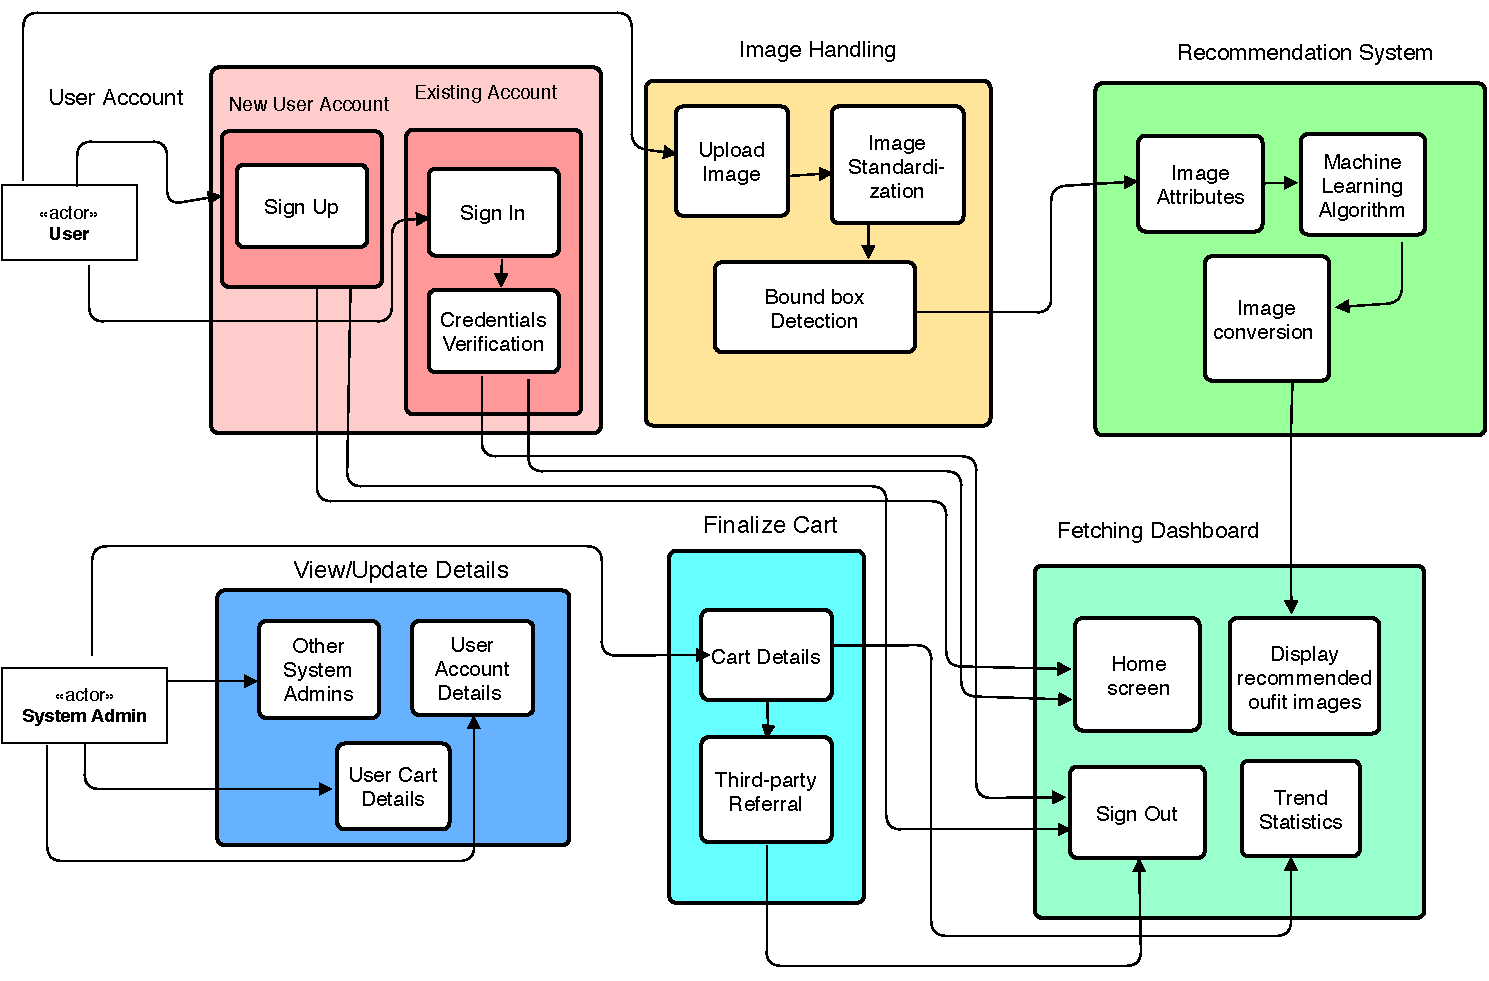
\includegraphics[width=15cm]{images/systemDiagram.pdf} 
\centering
\caption{Module-wise System Diagram}
\end{figure}

\section{Data Flow Diagram}
Rudimentary data flow diagrams for the system have also been constructed, given below:

\begin{figure}[ht]
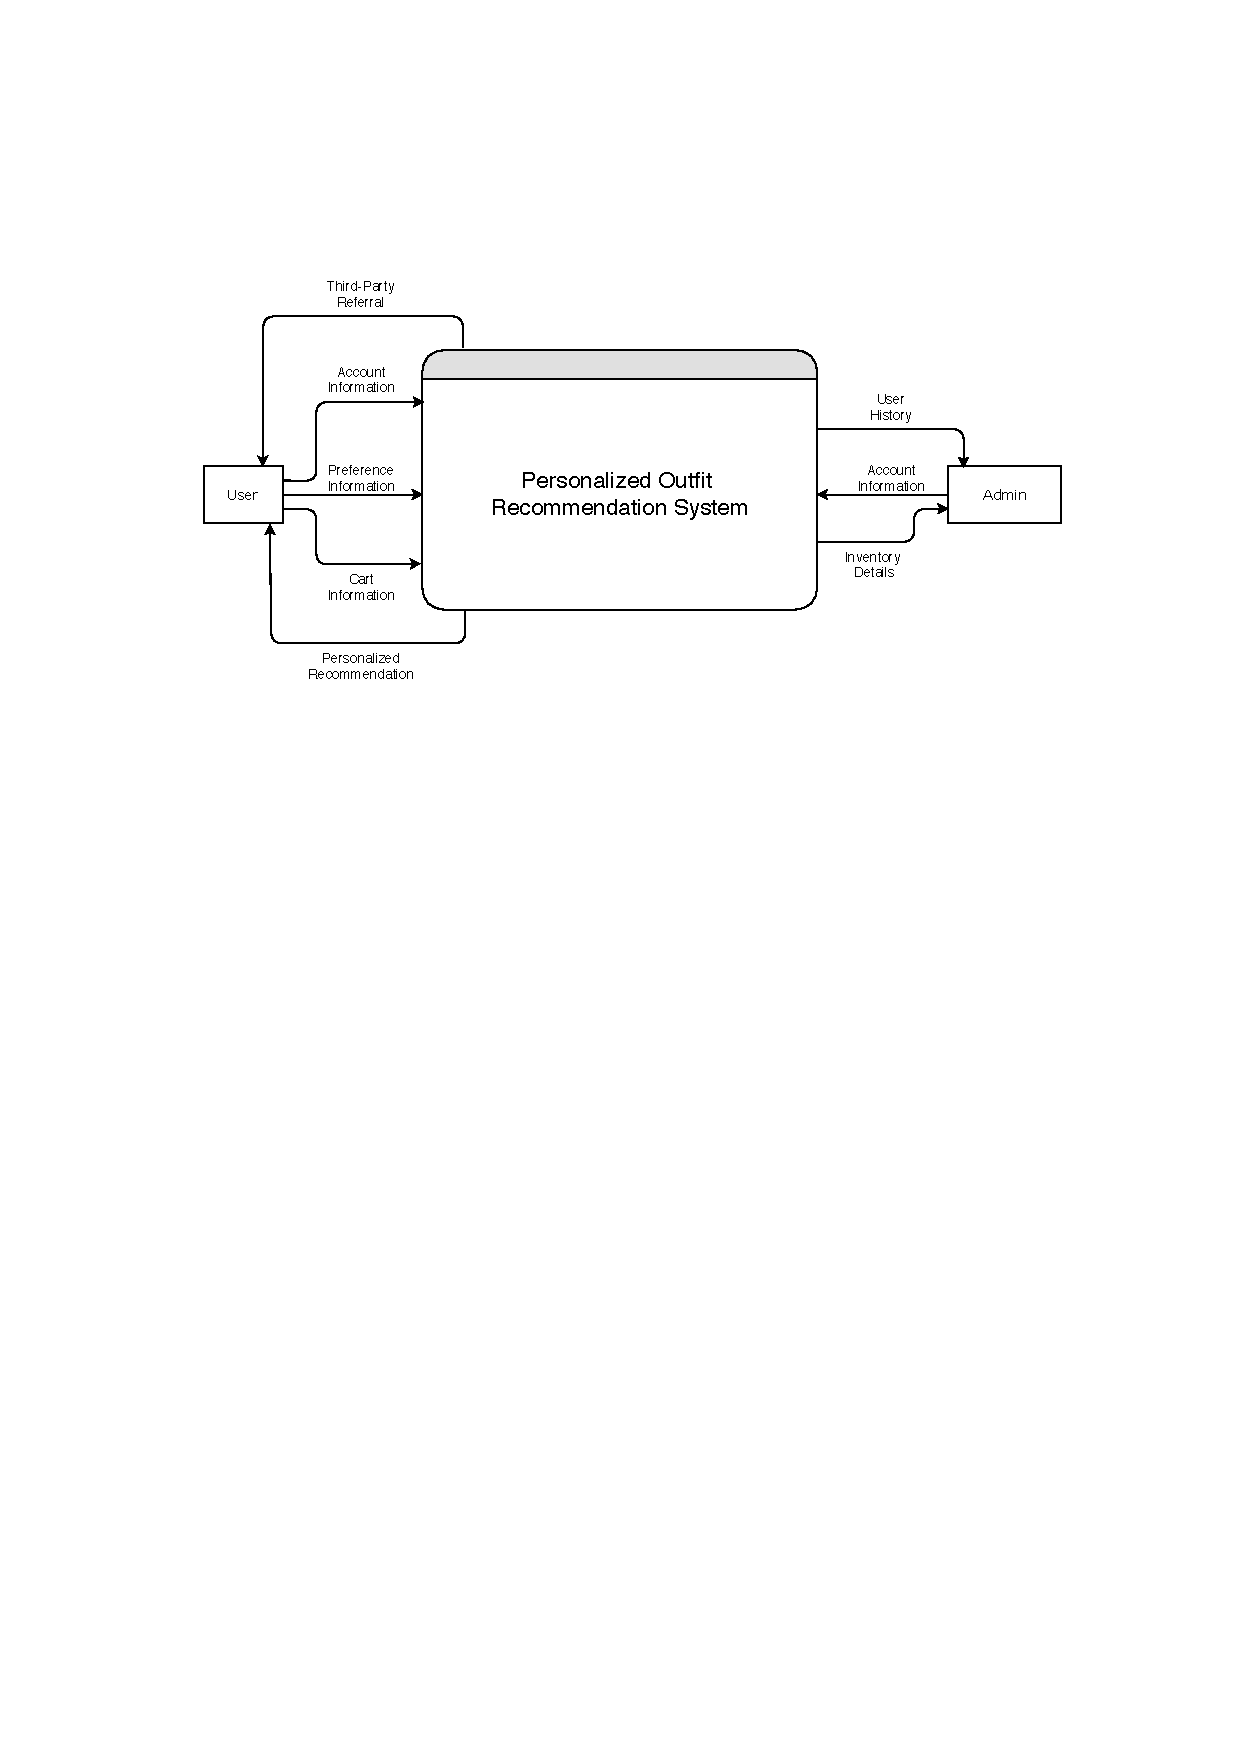
\includegraphics[width=15cm]{images/dfdContext.pdf} 
\centering
\caption{Context Level DFD}
\end{figure}

\begin{figure}[ht]
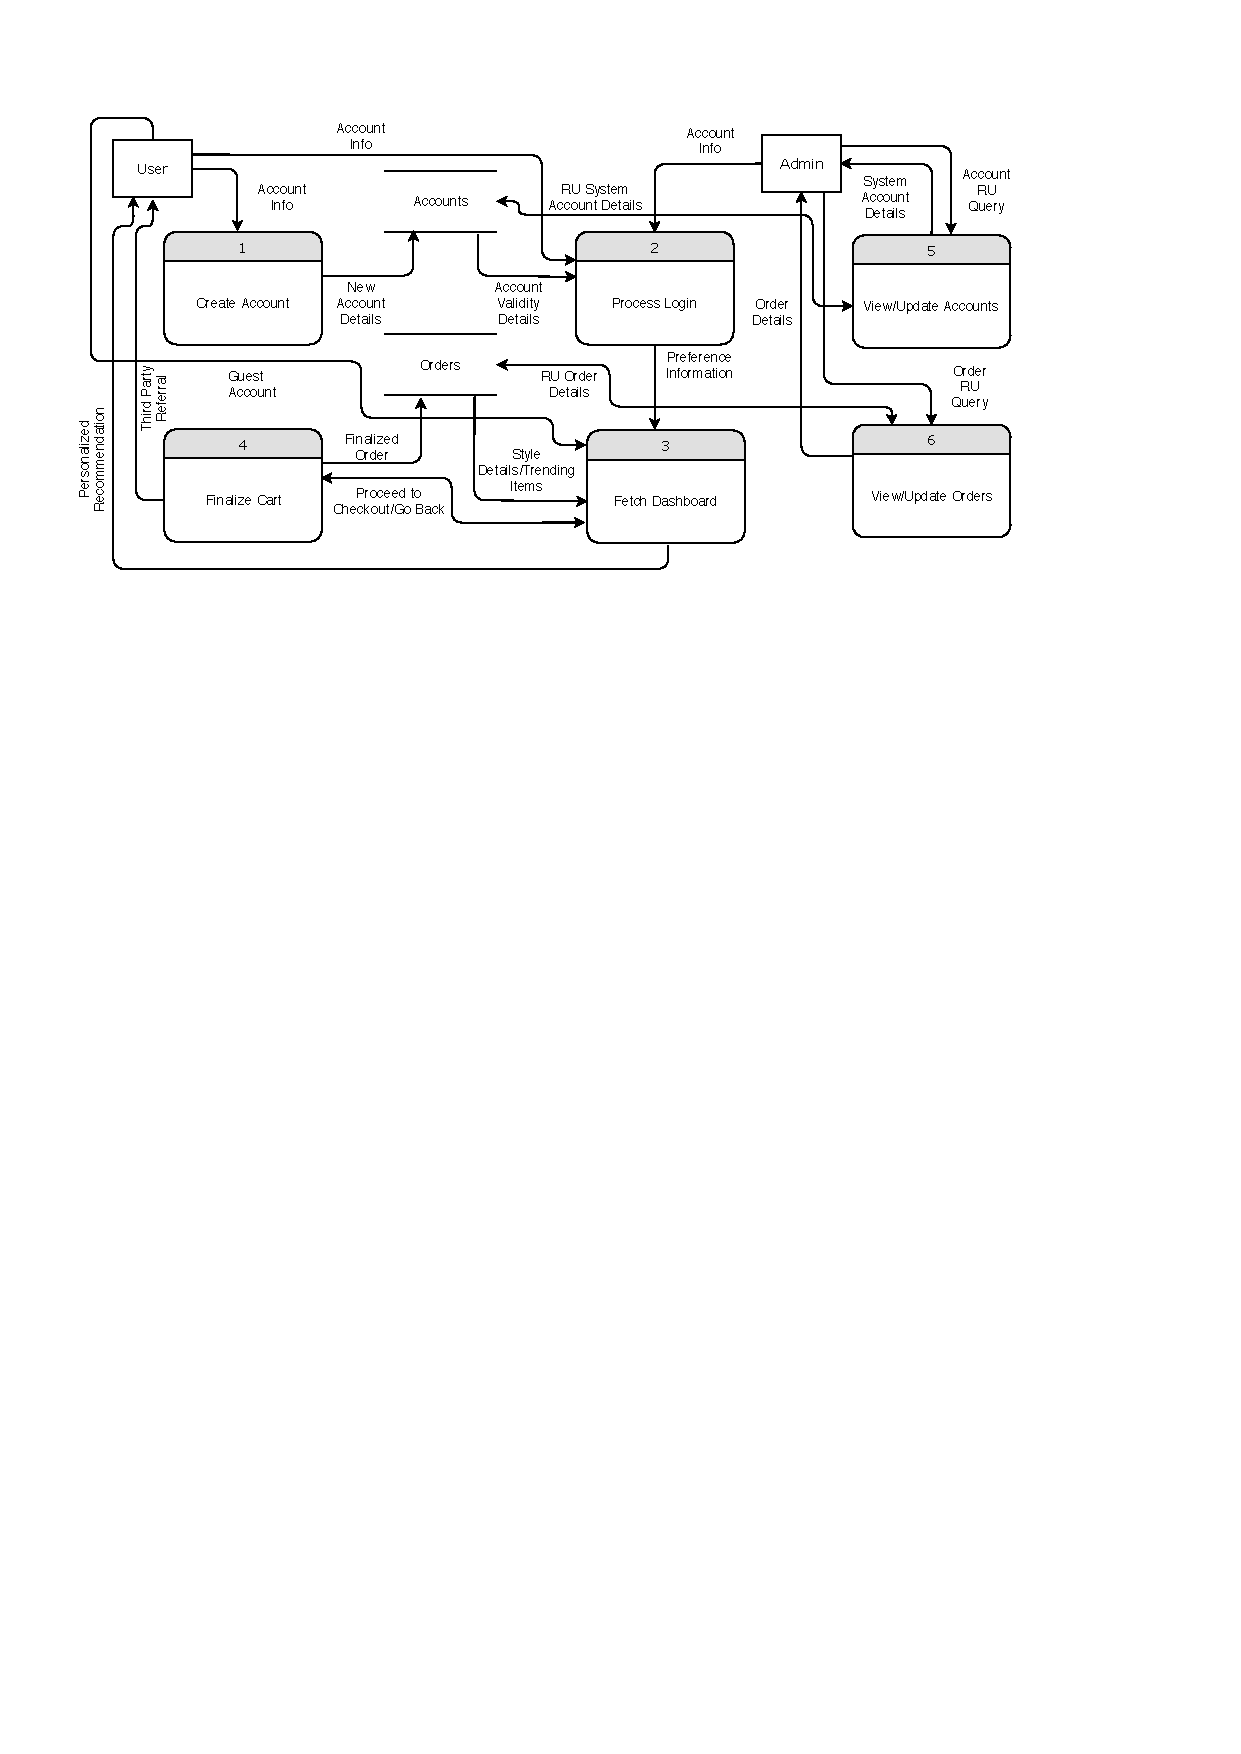
\includegraphics[width=15cm]{images/dfd0.pdf} 
\centering
\caption{0-Level DFD}
\end{figure}


\chapter{Software Design Specification (SDS)}
\label{chap:sds}
\input{chapters/sds}

\chapter{Experiments and Results}
\label{chap:results}
\input{chapters/results}

\chapter{Conclusion and Future Work}
\label{chap:outro}
\input{chapters/conclusion}

\begin{appendices}

\titleformat{\chapter}[hang]{\bf\huge}{Appendix \thechapter.}{2pc}{}
% \titleformat{\chapter}[hang]{\bf\huge}{\thechapter.}{2pc}{}

% This appendix is optional.
\chapter{More Math}
\input{chapters/appendix-math}

% This appendix is required if the data set is not fully described in the main text.
\chapter{Data}
\input{chapters/appendix-data}

% This appendix is required if the code is not fully described in the main text.
\chapter{Code}
\input{chapters/appendix-code}
\end{appendices}

% Print the bibliography with a ToC entry and titled, "References".
\printbibliography[heading=bibintoc,title={References}]

\end{document}

%%% Local Variables:
%%% mode: latex
%%% TeX-master: t
%%% End:
